% !TEX root = main.tex
\chapter{Overview of Research Triangle Park}
\label{Chapter:RTP}

In this chapter, we first define Research Triangle Park, the region studied in this thesis. We then explain why this region was chosen for this study, focusing on the rapid growth of the region and the significant presence of high tech companies and major universities.

\section{Where is Research Triangle Park?}
Research Triangle Park (RTP) is the largest research and science park in North America, and one of the largest in the world. The park, which stretches 7,000 acres across Wake and Durham counties was founded in 1959 by the Research Triangle Foundation. RTP is not a city, but it has its own special county district \cite{_research_????}. The Research Triangle Region Organization, a partnership dedicated to overseeing collaboration between businesses, government and various other institutions within the region identifies RTP as the following counties (see Figure \ref{fig:rtp-region}): Chatham, Durham, Edgecombe, Franklin, Granville, Harnett, Johnston, Lee, Moore, Nash, Orange, Person, Vance, Wake, Warren, and Wilson \cite{_research_????}. Additionally, the RTP Organization has stated that the RTP metro area has a population of 1.3 million people, and that there are 3 million people within a 60-mile radius of the park \cite{weddle_research_????}. Our project utilized public NC League of Municipalities (NCLM) data to identify all of the cities in each of the RTP counties to assist our research \cite{_north_????}.

\begin{figure}
\begin{center}
\resizebox{\textwidth}{!}{
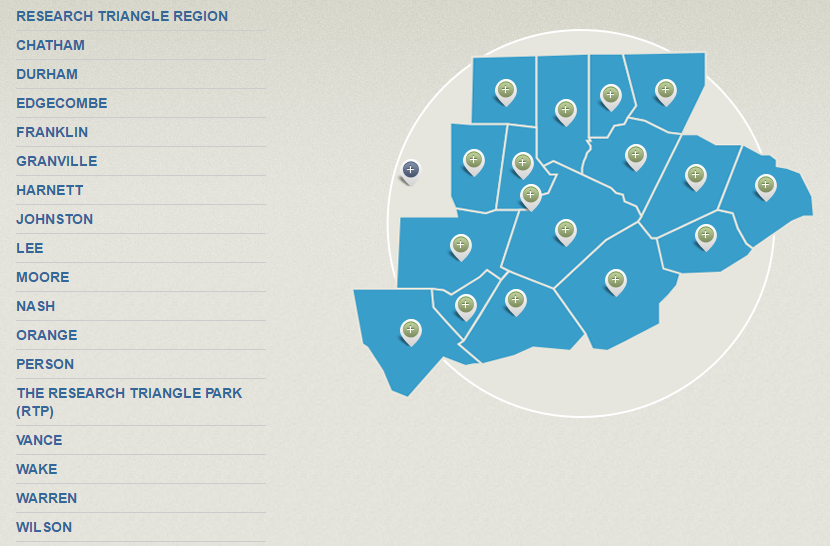
\includegraphics{Images/RTP-Region_2.png}
}
\caption{RTP region as defined by Research Triangle Region Organization \cite{_research_????}}
\label{fig:rtp-region}
\end{center}
\end{figure}

\section{Why Research Triangle Park?}

Many reasons can be attributed to our choosing of RTP and its surrounding communities for initial research into local open source activities. Over the last decade, numerous media outlets and journalists have continuously given this region nicknames such as “Start-up Capital of the South” \cite{_durhams_????} and “The Next Silicon Valley” \cite{_4_????}. Between 2000 and 2012, Raleigh's population grew 47.8 percent, which topped Forbes's list of fastest growing metropolitan areas in the country. This number was more than three times the overall growth of all other metropolitan areas \cite{kotkin_americas_????}. The Google for Entrepreneurs Network has invested in 3 different locations in Raleigh/Durham (RDU) for what they call "American Underground". American Underground is referred to as a "Start-Up Incubator" where software groups can rent space for their teams to meet and work \cite{_american_????}. The Research Triangle Park Organization continues to drive their mission to "change the course of history" by bringing people together and fostering innovation and creativity in the RTP community \cite{_research_2016}. They've recently open up a new center, The Frontier, with free space for teams to collaborate and participate in a variety of networking events \cite{_frontier_????}. 

Outside of the start-up communities, many big technology players have a presence in RTP--Red Hat, Citrix, Cisco, NetApp, IBM, Microsoft, Google, SAS, and others,  with more news about others following every year. There are several local prestigious universities including the University of North Carolina Chapel Hill, North Carolina State University, and Duke University, all of which are consistently producing top talent within the science, math and technology industries. According to the Research Triangle Park Organization \cite{_research_2016}, local companies and organizations have won Nobel Prizes and the Pulitzer. To date, they've recorded that there have been 245 company start-ups, 3,256 patents, and 1,970 trademarks. 

At the beginning of 2016, the North Carolina State of Technology Industry Report was released. We found some of the statistics produced by this group (NC Technology Association and Economic Leadership of Raleigh) relevant to reasons we chose the RTP region, even though they were specific to the state as a whole \cite{_nc_????}. 

A few of the highlights from this report included:

\begin{itemize}  
\item North Carolina is the \#2 state in Information Technology (IT) employment growth from 2009-2014.
\item North Carolina is the \#4 state for University Technology Licenses and Options Executed with 242 licenses and options in 2014.
\item Future North Carolina tech sector growth is expected to outpace national and American South averages.
\item Over the past year technology employment grew by 3.6 percent, and technology establishments grew by 5.2 percent.
\end{itemize}

These statistics can serve as a proxy for choosing to do research on other areas with a large and growing presence in the information technology industry.
